\documentclass[1p]{elsarticle_modified}
%\bibliographystyle{elsarticle-num}

%\usepackage[colorlinks]{hyperref}
%\usepackage{abbrmath_seonhwa} %\Abb, \Ascr, \Acal ,\Abf, \Afrak
\usepackage{amsfonts}
\usepackage{amssymb}
\usepackage{amsmath}
\usepackage{amsthm}
\usepackage{scalefnt}
\usepackage{amsbsy}
\usepackage{kotex}
\usepackage{caption}
\usepackage{subfig}
\usepackage{color}
\usepackage{graphicx}
\usepackage{xcolor} %% white, black, red, green, blue, cyan, magenta, yellow
\usepackage{float}
\usepackage{setspace}
\usepackage{hyperref}

\usepackage{tikz}
\usetikzlibrary{arrows}

\usepackage{multirow}
\usepackage{array} % fixed length table
\usepackage{hhline}

%%%%%%%%%%%%%%%%%%%%%
\makeatletter
\renewcommand*\env@matrix[1][\arraystretch]{%
	\edef\arraystretch{#1}%
	\hskip -\arraycolsep
	\let\@ifnextchar\new@ifnextchar
	\array{*\c@MaxMatrixCols c}}
\makeatother %https://tex.stackexchange.com/questions/14071/how-can-i-increase-the-line-spacing-in-a-matrix
%%%%%%%%%%%%%%%

\usepackage[normalem]{ulem}

\newcommand{\msout}[1]{\ifmmode\text{\sout{\ensuremath{#1}}}\else\sout{#1}\fi}
%SOURCE: \msout is \stkout macro in https://tex.stackexchange.com/questions/20609/strikeout-in-math-mode

\newcommand{\cancel}[1]{
	\ifmmode
	{\color{red}\msout{#1}}
	\else
	{\color{red}\sout{#1}}
	\fi
}

\newcommand{\add}[1]{
	{\color{blue}\uwave{#1}}
}

\newcommand{\replace}[2]{
	\ifmmode
	{\color{red}\msout{#1}}{\color{blue}\uwave{#2}}
	\else
	{\color{red}\sout{#1}}{\color{blue}\uwave{#2}}
	\fi
}

\newcommand{\Sol}{\mathcal{S}} %segment
\newcommand{\D}{D} %diagram
\newcommand{\A}{\mathcal{A}} %arc


%%%%%%%%%%%%%%%%%%%%%%%%%%%%%5 test

\def\sl{\operatorname{\textup{SL}}(2,\Cbb)}
\def\psl{\operatorname{\textup{PSL}}(2,\Cbb)}
\def\quan{\mkern 1mu \triangleright \mkern 1mu}

\theoremstyle{definition}
\newtheorem{thm}{Theorem}[section]
\newtheorem{prop}[thm]{Proposition}
\newtheorem{lem}[thm]{Lemma}
\newtheorem{ques}[thm]{Question}
\newtheorem{cor}[thm]{Corollary}
\newtheorem{defn}[thm]{Definition}
\newtheorem{exam}[thm]{Example}
\newtheorem{rmk}[thm]{Remark}
\newtheorem{alg}[thm]{Algorithm}

\newcommand{\I}{\sqrt{-1}}
\begin{document}

%\begin{frontmatter}
%
%\title{Boundary parabolic representations of knots up to 8 crossings}
%
%%% Group authors per affiliation:
%\author{Yunhi Cho} 
%\address{Department of Mathematics, University of Seoul, Seoul, Korea}
%\ead{yhcho@uos.ac.kr}
%
%
%\author{Seonhwa Kim} %\fnref{s_kim}}
%\address{Center for Geometry and Physics, Institute for Basic Science, Pohang, 37673, Korea}
%\ead{ryeona17@ibs.re.kr}
%
%\author{Hyuk Kim}
%\address{Department of Mathematical Sciences, Seoul National University, Seoul 08826, Korea}
%\ead{hyukkim@snu.ac.kr}
%
%\author{Seokbeom Yoon}
%\address{Department of Mathematical Sciences, Seoul National University, Seoul, 08826,  Korea}
%\ead{sbyoon15@snu.ac.kr}
%
%\begin{abstract}
%We find all boundary parabolic representation of knots up to 8 crossings.
%
%\end{abstract}
%\begin{keyword}
%    \MSC[2010] 57M25 
%\end{keyword}
%
%\end{frontmatter}

%\linenumbers
%\tableofcontents
%
\newcommand\colored[1]{\textcolor{white}{\rule[-0.35ex]{0.8em}{1.4ex}}\kern-0.8em\color{red} #1}%
%\newcommand\colored[1]{\textcolor{white}{ #1}\kern-2.17ex	\textcolor{white}{ #1}\kern-1.81ex	\textcolor{white}{ #1}\kern-2.15ex\color{red}#1	}

{\Large $\underline{12n_{0367}~(K12n_{0367})}$}

\setlength{\tabcolsep}{10pt}
\renewcommand{\arraystretch}{1.6}
\vspace{1cm}\begin{tabular}{m{100pt}>{\centering\arraybackslash}m{274pt}}
\multirow{5}{120pt}{
	\centering
	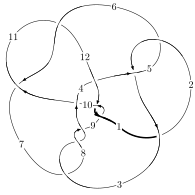
\includegraphics[width=112pt]{../../../GIT/diagram.site/Diagrams/png/2456_12n_0367.png}\\
\ \ \ A knot diagram\footnotemark}&
\allowdisplaybreaks
\textbf{Linearized knot diagam} \\
\cline{2-2}
 &
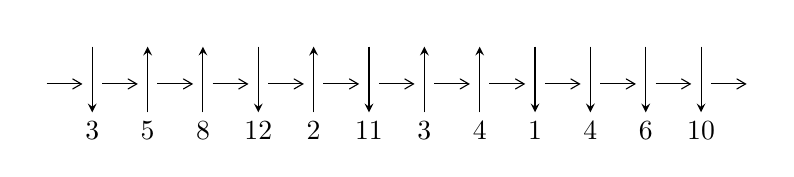
\begin{tikzpicture}[x=20pt, y=17pt]
	% nodes
	\node (C0) at (0, 0) {};
	\node (C1) at (1, 0) {};
	\node (C1U) at (1, +1) {};
	\node (C1D) at (1, -1) {3};

	\node (C2) at (2, 0) {};
	\node (C2U) at (2, +1) {};
	\node (C2D) at (2, -1) {5};

	\node (C3) at (3, 0) {};
	\node (C3U) at (3, +1) {};
	\node (C3D) at (3, -1) {8};

	\node (C4) at (4, 0) {};
	\node (C4U) at (4, +1) {};
	\node (C4D) at (4, -1) {12};

	\node (C5) at (5, 0) {};
	\node (C5U) at (5, +1) {};
	\node (C5D) at (5, -1) {2};

	\node (C6) at (6, 0) {};
	\node (C6U) at (6, +1) {};
	\node (C6D) at (6, -1) {11};

	\node (C7) at (7, 0) {};
	\node (C7U) at (7, +1) {};
	\node (C7D) at (7, -1) {3};

	\node (C8) at (8, 0) {};
	\node (C8U) at (8, +1) {};
	\node (C8D) at (8, -1) {4};

	\node (C9) at (9, 0) {};
	\node (C9U) at (9, +1) {};
	\node (C9D) at (9, -1) {1};

	\node (C10) at (10, 0) {};
	\node (C10U) at (10, +1) {};
	\node (C10D) at (10, -1) {4};

	\node (C11) at (11, 0) {};
	\node (C11U) at (11, +1) {};
	\node (C11D) at (11, -1) {6};

	\node (C12) at (12, 0) {};
	\node (C12U) at (12, +1) {};
	\node (C12D) at (12, -1) {10};
	\node (C13) at (13, 0) {};

	% arrows
	\draw[->,>={angle 60}]
	(C0) edge (C1) (C1) edge (C2) (C2) edge (C3) (C3) edge (C4) (C4) edge (C5) (C5) edge (C6) (C6) edge (C7) (C7) edge (C8) (C8) edge (C9) (C9) edge (C10) (C10) edge (C11) (C11) edge (C12) (C12) edge (C13) ;	\draw[->,>=stealth]
	(C1U) edge (C1D) (C2D) edge (C2U) (C3D) edge (C3U) (C4U) edge (C4D) (C5D) edge (C5U) (C6U) edge (C6D) (C7D) edge (C7U) (C8D) edge (C8U) (C9U) edge (C9D) (C10U) edge (C10D) (C11U) edge (C11D) (C12U) edge (C12D) ;
	\end{tikzpicture} \\
\hhline{~~} \\& 
\textbf{Solving Sequence} \\ \cline{2-2} 
 &
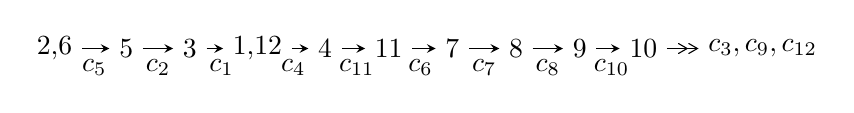
\begin{tikzpicture}[x=23pt, y=7pt]
	% node
	\node (A0) at (-1/8, 0) {2,6};
	\node (A1) at (1, 0) {5};
	\node (A2) at (2, 0) {3};
	\node (A3) at (49/16, 0) {1,12};
	\node (A4) at (33/8, 0) {4};
	\node (A5) at (41/8, 0) {11};
	\node (A6) at (49/8, 0) {7};
	\node (A7) at (57/8, 0) {8};
	\node (A8) at (65/8, 0) {9};
	\node (A9) at (73/8, 0) {10};
	\node (C1) at (1/2, -1) {$c_{5}$};
	\node (C2) at (3/2, -1) {$c_{2}$};
	\node (C3) at (5/2, -1) {$c_{1}$};
	\node (C4) at (29/8, -1) {$c_{4}$};
	\node (C5) at (37/8, -1) {$c_{11}$};
	\node (C6) at (45/8, -1) {$c_{6}$};
	\node (C7) at (53/8, -1) {$c_{7}$};
	\node (C8) at (61/8, -1) {$c_{8}$};
	\node (C9) at (69/8, -1) {$c_{10}$};
	\node (A10) at (11, 0) {$c_{3},c_{9},c_{12}$};

	% edge
	\draw[->,>=stealth]	
	(A0) edge (A1) (A1) edge (A2) (A2) edge (A3) (A3) edge (A4) (A4) edge (A5) (A5) edge (A6) (A6) edge (A7) (A7) edge (A8) (A8) edge (A9) ;
	\draw[->>,>={angle 60}]	
	(A9) edge (A10);
\end{tikzpicture} \\ 

\end{tabular} \\

\footnotetext{
The image of knot diagram is generated by the software ``\textbf{Draw programme}" developed by Andrew Bartholomew(\url{http://www.layer8.co.uk/maths/draw/index.htm\#Running-draw}), where we modified some parts for our purpose(\url{https://github.com/CATsTAILs/LinksPainter}).
}\phantom \\ \newline 
\centering \textbf{Ideals for irreducible components\footnotemark of $X_{\text{par}}$} 
 
\begin{align*}
I^u_{1}&=\langle 
-1.53963\times10^{157} u^{87}+2.37834\times10^{157} u^{86}+\cdots+2.39381\times10^{157} b+1.76070\times10^{157},\\
\phantom{I^u_{1}}&\phantom{= \langle  }2.34713\times10^{157} u^{87}-1.38197\times10^{157} u^{86}+\cdots+2.39381\times10^{157} a+1.30597\times10^{158},\;u^{88}+22 u^{86}+\cdots+2 u+1\rangle \\
I^u_{2}&=\langle 
-104670 u^{25}+66491 u^{24}+\cdots+54833 b-636383,\\
\phantom{I^u_{2}}&\phantom{= \langle  }495202 u^{25}-847689 u^{24}+\cdots+54833 a+692536,\;u^{26}-3 u^{25}+\cdots-3 u+1\rangle \\
\\
\end{align*}
\raggedright * 2 irreducible components of $\dim_{\mathbb{C}}=0$, with total 114 representations.\\
\footnotetext{All coefficients of polynomials are rational numbers. But the coefficients are sometimes approximated in decimal forms when there is not enough margin.}
\newpage
\renewcommand{\arraystretch}{1}
\centering \section*{I. $I^u_{1}= \langle -1.54\times10^{157} u^{87}+2.38\times10^{157} u^{86}+\cdots+2.39\times10^{157} b+1.76\times10^{157},\;2.35\times10^{157} u^{87}-1.38\times10^{157} u^{86}+\cdots+2.39\times10^{157} a+1.31\times10^{158},\;u^{88}+22 u^{86}+\cdots+2 u+1 \rangle$}
\flushleft \textbf{(i) Arc colorings}\\
\begin{tabular}{m{7pt} m{180pt} m{7pt} m{180pt} }
\flushright $a_{2}=$&$\begin{pmatrix}0\\u\end{pmatrix}$ \\
\flushright $a_{6}=$&$\begin{pmatrix}1\\0\end{pmatrix}$ \\
\flushright $a_{5}=$&$\begin{pmatrix}1\\u^2\end{pmatrix}$ \\
\flushright $a_{3}=$&$\begin{pmatrix}u\\u^3+u\end{pmatrix}$ \\
\flushright $a_{1}=$&$\begin{pmatrix}u^3\\u^5+u^3+u\end{pmatrix}$ \\
\flushright $a_{12}=$&$\begin{pmatrix}-0.980503 u^{87}+0.577312 u^{86}+\cdots-5.19109 u-5.45563\\0.643174 u^{87}-0.993539 u^{86}+\cdots+2.61924 u-0.735525\end{pmatrix}$ \\
\flushright $a_{4}=$&$\begin{pmatrix}-1.71029 u^{87}+0.0126145 u^{86}+\cdots+6.15889 u-0.333775\\0.314661 u^{87}-0.105993 u^{86}+\cdots+1.28030 u+0.137825\end{pmatrix}$ \\
\flushright $a_{11}=$&$\begin{pmatrix}-0.337329 u^{87}-0.416227 u^{86}+\cdots-2.57184 u-6.19116\\0.643174 u^{87}-0.993539 u^{86}+\cdots+2.61924 u-0.735525\end{pmatrix}$ \\
\flushright $a_{7}=$&$\begin{pmatrix}1.33512 u^{87}+0.213674 u^{86}+\cdots-8.43237 u+2.51339\\-0.537763 u^{87}+0.298042 u^{86}+\cdots-2.98445 u-0.0534571\end{pmatrix}$ \\
\flushright $a_{8}=$&$\begin{pmatrix}1.40782 u^{87}+0.124868 u^{86}+\cdots-7.03532 u+2.37329\\-0.415885 u^{87}+0.204932 u^{86}+\cdots-1.48248 u-0.104746\end{pmatrix}$ \\
\flushright $a_{9}=$&$\begin{pmatrix}-0.297558 u^{87}+0.610697 u^{86}+\cdots-1.00875 u+4.31265\\-0.434217 u^{87}+0.436621 u^{86}+\cdots-1.53241 u+0.242672\end{pmatrix}$ \\
\flushright $a_{10}=$&$\begin{pmatrix}0.195621 u^{87}-0.814050 u^{86}+\cdots+0.450308 u-4.69598\\0.281328 u^{87}-0.153582 u^{86}+\cdots+2.43945 u+0.00833811\end{pmatrix}$\\&\end{tabular}
\flushleft \textbf{(ii) Obstruction class $= -1$}\\~\\
\flushleft \textbf{(iii) Cusp Shapes $= -1.98512 u^{87}+0.111068 u^{86}+\cdots+1.77043 u-2.63654$}\\~\\
\newpage\renewcommand{\arraystretch}{1}
\flushleft \textbf{(iv) u-Polynomials at the component}\newline \\
\begin{tabular}{m{50pt}|m{274pt}}
Crossings & \hspace{64pt}u-Polynomials at each crossing \\
\hline $$\begin{aligned}c_{1}\end{aligned}$$&$\begin{aligned}
&u^{88}+44 u^{87}+\cdots-14 u+1
\end{aligned}$\\
\hline $$\begin{aligned}c_{2},c_{5}\end{aligned}$$&$\begin{aligned}
&u^{88}+22 u^{86}+\cdots+2 u+1
\end{aligned}$\\
\hline $$\begin{aligned}c_{3},c_{7},c_{8}\end{aligned}$$&$\begin{aligned}
&u^{88}+u^{87}+\cdots+4537 u+653
\end{aligned}$\\
\hline $$\begin{aligned}c_{4}\end{aligned}$$&$\begin{aligned}
&u^{88}+u^{87}+\cdots-6282 u+3780
\end{aligned}$\\
\hline $$\begin{aligned}c_{6},c_{11}\end{aligned}$$&$\begin{aligned}
&u^{88}-3 u^{87}+\cdots-34779 u+4553
\end{aligned}$\\
\hline $$\begin{aligned}c_{9},c_{12}\end{aligned}$$&$\begin{aligned}
&u^{88}-3 u^{87}+\cdots-5791 u+1003
\end{aligned}$\\
\hline $$\begin{aligned}c_{10}\end{aligned}$$&$\begin{aligned}
&u^{88}- u^{87}+\cdots+33861 u+11617
\end{aligned}$\\
\hline
\end{tabular}\\~\\
\newpage\renewcommand{\arraystretch}{1}
\flushleft \textbf{(v) Riley Polynomials at the component}\newline \\
\begin{tabular}{m{50pt}|m{274pt}}
Crossings & \hspace{64pt}Riley Polynomials at each crossing \\
\hline $$\begin{aligned}c_{1}\end{aligned}$$&$\begin{aligned}
&y^{88}+16 y^{87}+\cdots+38 y+1
\end{aligned}$\\
\hline $$\begin{aligned}c_{2},c_{5}\end{aligned}$$&$\begin{aligned}
&y^{88}+44 y^{87}+\cdots-14 y+1
\end{aligned}$\\
\hline $$\begin{aligned}c_{3},c_{7},c_{8}\end{aligned}$$&$\begin{aligned}
&y^{88}-39 y^{87}+\cdots-16718609 y+426409
\end{aligned}$\\
\hline $$\begin{aligned}c_{4}\end{aligned}$$&$\begin{aligned}
&y^{88}+47 y^{87}+\cdots+424002276 y+14288400
\end{aligned}$\\
\hline $$\begin{aligned}c_{6},c_{11}\end{aligned}$$&$\begin{aligned}
&y^{88}+47 y^{87}+\cdots+457119657 y+20729809
\end{aligned}$\\
\hline $$\begin{aligned}c_{9},c_{12}\end{aligned}$$&$\begin{aligned}
&y^{88}+37 y^{87}+\cdots+28963255 y+1006009
\end{aligned}$\\
\hline $$\begin{aligned}c_{10}\end{aligned}$$&$\begin{aligned}
&y^{88}-13 y^{87}+\cdots-5986209521 y+134954689
\end{aligned}$\\
\hline
\end{tabular}\\~\\
\newpage\flushleft \textbf{(vi) Complex Volumes and Cusp Shapes}
$$\begin{array}{c|c|c}  
\text{Solutions to }I^u_{1}& \I (\text{vol} + \sqrt{-1}CS) & \text{Cusp shape}\\
 \hline 
\begin{aligned}
u &= \phantom{-}0.950994 + 0.225023 I \\
a &= -0.0042485 + 0.1234880 I \\
b &= -0.494741 - 1.159590 I\end{aligned}
 & \phantom{-}2.20661 - 4.50051 I & \phantom{-0.000000 } 0 \\ \hline\begin{aligned}
u &= \phantom{-}0.950994 - 0.225023 I \\
a &= -0.0042485 - 0.1234880 I \\
b &= -0.494741 + 1.159590 I\end{aligned}
 & \phantom{-}2.20661 + 4.50051 I & \phantom{-0.000000 } 0 \\ \hline\begin{aligned}
u &= \phantom{-}0.285666 + 0.999025 I \\
a &= -1.271540 - 0.078839 I \\
b &= \phantom{-}0.527665 + 0.001231 I\end{aligned}
 & -0.94739 + 2.27872 I & \phantom{-0.000000 } 0 \\ \hline\begin{aligned}
u &= \phantom{-}0.285666 - 0.999025 I \\
a &= -1.271540 + 0.078839 I \\
b &= \phantom{-}0.527665 - 0.001231 I\end{aligned}
 & -0.94739 - 2.27872 I & \phantom{-0.000000 } 0 \\ \hline\begin{aligned}
u &= -0.925529 + 0.492184 I \\
a &= -0.0605045 + 0.0712789 I \\
b &= -0.599977 + 1.165180 I\end{aligned}
 & \phantom{-}1.40800 + 4.49923 I & \phantom{-0.000000 } 0 \\ \hline\begin{aligned}
u &= -0.925529 - 0.492184 I \\
a &= -0.0605045 - 0.0712789 I \\
b &= -0.599977 - 1.165180 I\end{aligned}
 & \phantom{-}1.40800 - 4.49923 I & \phantom{-0.000000 } 0 \\ \hline\begin{aligned}
u &= -0.432052 + 0.965201 I \\
a &= \phantom{-}2.14505 + 0.62032 I \\
b &= -0.210712 - 1.326370 I\end{aligned}
 & \phantom{-}4.71577 - 4.97810 I & \phantom{-0.000000 } 0 \\ \hline\begin{aligned}
u &= -0.432052 - 0.965201 I \\
a &= \phantom{-}2.14505 - 0.62032 I \\
b &= -0.210712 + 1.326370 I\end{aligned}
 & \phantom{-}4.71577 + 4.97810 I & \phantom{-0.000000 } 0 \\ \hline\begin{aligned}
u &= \phantom{-}0.403742 + 0.986207 I \\
a &= \phantom{-}1.42705 + 0.78190 I \\
b &= -1.24697 - 0.68296 I\end{aligned}
 & -2.68120 + 2.73860 I & \phantom{-0.000000 } 0 \\ \hline\begin{aligned}
u &= \phantom{-}0.403742 - 0.986207 I \\
a &= \phantom{-}1.42705 - 0.78190 I \\
b &= -1.24697 + 0.68296 I\end{aligned}
 & -2.68120 - 2.73860 I & \phantom{-0.000000 } 0\\
 \hline 
 \end{array}$$\newpage$$\begin{array}{c|c|c}  
\text{Solutions to }I^u_{1}& \I (\text{vol} + \sqrt{-1}CS) & \text{Cusp shape}\\
 \hline 
\begin{aligned}
u &= -0.495500 + 0.945563 I \\
a &= -1.87127 - 0.61725 I \\
b &= \phantom{-}0.44695 + 1.42224 I\end{aligned}
 & \phantom{-}5.23357 - 0.17704 I & \phantom{-0.000000 } 0 \\ \hline\begin{aligned}
u &= -0.495500 - 0.945563 I \\
a &= -1.87127 + 0.61725 I \\
b &= \phantom{-}0.44695 - 1.42224 I\end{aligned}
 & \phantom{-}5.23357 + 0.17704 I & \phantom{-0.000000 } 0 \\ \hline\begin{aligned}
u &= \phantom{-}0.916402 + 0.070900 I \\
a &= -0.293096 - 0.421980 I \\
b &= \phantom{-}0.038009 - 1.374640 I\end{aligned}
 & \phantom{-}6.89951 + 0.18727 I & \phantom{-}7.38962 + 0. I\phantom{ +0.000000I} \\ \hline\begin{aligned}
u &= \phantom{-}0.916402 - 0.070900 I \\
a &= -0.293096 + 0.421980 I \\
b &= \phantom{-}0.038009 + 1.374640 I\end{aligned}
 & \phantom{-}6.89951 - 0.18727 I & \phantom{-}7.38962 + 0. I\phantom{ +0.000000I} \\ \hline\begin{aligned}
u &= -0.362440 + 1.049730 I \\
a &= \phantom{-}1.47595 - 0.54699 I \\
b &= -0.685813 - 0.954186 I\end{aligned}
 & -4.05142 - 3.40776 I & \phantom{-0.000000 } 0 \\ \hline\begin{aligned}
u &= -0.362440 - 1.049730 I \\
a &= \phantom{-}1.47595 + 0.54699 I \\
b &= -0.685813 + 0.954186 I\end{aligned}
 & -4.05142 + 3.40776 I & \phantom{-0.000000 } 0 \\ \hline\begin{aligned}
u &= \phantom{-}0.830410 + 0.267292 I \\
a &= -0.154904 - 0.043619 I \\
b &= \phantom{-}0.434261 + 0.771534 I\end{aligned}
 & \phantom{-}1.041510 + 0.827983 I & \phantom{-}1.47393 - 1.48857 I \\ \hline\begin{aligned}
u &= \phantom{-}0.830410 - 0.267292 I \\
a &= -0.154904 + 0.043619 I \\
b &= \phantom{-}0.434261 - 0.771534 I\end{aligned}
 & \phantom{-}1.041510 - 0.827983 I & \phantom{-}1.47393 + 1.48857 I \\ \hline\begin{aligned}
u &= -0.482044 + 0.714046 I \\
a &= \phantom{-}0.501977 + 0.389736 I \\
b &= \phantom{-}0.18713 - 1.65749 I\end{aligned}
 & \phantom{-}5.99785 - 3.85058 I & \phantom{-}2.05614 + 7.78115 I \\ \hline\begin{aligned}
u &= -0.482044 - 0.714046 I \\
a &= \phantom{-}0.501977 - 0.389736 I \\
b &= \phantom{-}0.18713 + 1.65749 I\end{aligned}
 & \phantom{-}5.99785 + 3.85058 I & \phantom{-}2.05614 - 7.78115 I\\
 \hline 
 \end{array}$$\newpage$$\begin{array}{c|c|c}  
\text{Solutions to }I^u_{1}& \I (\text{vol} + \sqrt{-1}CS) & \text{Cusp shape}\\
 \hline 
\begin{aligned}
u &= \phantom{-}0.530443 + 1.007740 I \\
a &= \phantom{-}0.833164 + 0.920449 I \\
b &= -0.421505 + 1.042970 I\end{aligned}
 & -1.79639 + 3.12241 I & \phantom{-0.000000 } 0 \\ \hline\begin{aligned}
u &= \phantom{-}0.530443 - 1.007740 I \\
a &= \phantom{-}0.833164 - 0.920449 I \\
b &= -0.421505 - 1.042970 I\end{aligned}
 & -1.79639 - 3.12241 I & \phantom{-0.000000 } 0 \\ \hline\begin{aligned}
u &= -0.289666 + 1.102280 I \\
a &= -1.158050 + 0.650210 I \\
b &= \phantom{-}0.606326 + 0.743837 I\end{aligned}
 & -3.08768 + 2.63543 I & \phantom{-0.000000 } 0 \\ \hline\begin{aligned}
u &= -0.289666 - 1.102280 I \\
a &= -1.158050 - 0.650210 I \\
b &= \phantom{-}0.606326 - 0.743837 I\end{aligned}
 & -3.08768 - 2.63543 I & \phantom{-0.000000 } 0 \\ \hline\begin{aligned}
u &= -1.070320 + 0.410063 I \\
a &= -0.0461963 - 0.0452036 I \\
b &= \phantom{-}0.560313 - 1.284340 I\end{aligned}
 & \phantom{-}4.31681 + 10.86790 I & \phantom{-0.000000 } 0 \\ \hline\begin{aligned}
u &= -1.070320 - 0.410063 I \\
a &= -0.0461963 + 0.0452036 I \\
b &= \phantom{-}0.560313 + 1.284340 I\end{aligned}
 & \phantom{-}4.31681 - 10.86790 I & \phantom{-0.000000 } 0 \\ \hline\begin{aligned}
u &= -0.443590 + 1.065640 I \\
a &= \phantom{-}1.65905 + 1.05131 I \\
b &= -0.161908 - 0.797457 I\end{aligned}
 & \phantom{-}6.47178 - 2.16309 I & \phantom{-0.000000 } 0 \\ \hline\begin{aligned}
u &= -0.443590 - 1.065640 I \\
a &= \phantom{-}1.65905 - 1.05131 I \\
b &= -0.161908 + 0.797457 I\end{aligned}
 & \phantom{-}6.47178 + 2.16309 I & \phantom{-0.000000 } 0 \\ \hline\begin{aligned}
u &= \phantom{-}0.382878 + 1.090750 I \\
a &= -1.010260 - 0.717946 I \\
b &= \phantom{-}0.944931 + 0.886998 I\end{aligned}
 & -2.05368 - 1.85448 I & \phantom{-0.000000 } 0 \\ \hline\begin{aligned}
u &= \phantom{-}0.382878 - 1.090750 I \\
a &= -1.010260 + 0.717946 I \\
b &= \phantom{-}0.944931 - 0.886998 I\end{aligned}
 & -2.05368 + 1.85448 I & \phantom{-0.000000 } 0\\
 \hline 
 \end{array}$$\newpage$$\begin{array}{c|c|c}  
\text{Solutions to }I^u_{1}& \I (\text{vol} + \sqrt{-1}CS) & \text{Cusp shape}\\
 \hline 
\begin{aligned}
u &= \phantom{-}0.260391 + 0.792542 I \\
a &= \phantom{-}2.02389 + 0.11691 I \\
b &= -1.214820 - 0.002643 I\end{aligned}
 & -1.73937 + 0.22136 I & \phantom{-}1.85602 + 1.46273 I \\ \hline\begin{aligned}
u &= \phantom{-}0.260391 - 0.792542 I \\
a &= \phantom{-}2.02389 - 0.11691 I \\
b &= -1.214820 + 0.002643 I\end{aligned}
 & -1.73937 - 0.22136 I & \phantom{-}1.85602 - 1.46273 I \\ \hline\begin{aligned}
u &= -0.528314 + 1.040610 I \\
a &= \phantom{-}0.932239 - 0.854300 I \\
b &= -1.269650 + 0.553169 I\end{aligned}
 & -2.98847 - 3.16275 I & \phantom{-0.000000 } 0 \\ \hline\begin{aligned}
u &= -0.528314 - 1.040610 I \\
a &= \phantom{-}0.932239 + 0.854300 I \\
b &= -1.269650 - 0.553169 I\end{aligned}
 & -2.98847 + 3.16275 I & \phantom{-0.000000 } 0 \\ \hline\begin{aligned}
u &= -0.396057 + 0.732711 I \\
a &= -0.617862 + 0.433950 I \\
b &= -0.07362 + 1.57635 I\end{aligned}
 & \phantom{-}5.53692 + 1.45907 I & \phantom{-}2.09471 + 3.45616 I \\ \hline\begin{aligned}
u &= -0.396057 - 0.732711 I \\
a &= -0.617862 - 0.433950 I \\
b &= -0.07362 - 1.57635 I\end{aligned}
 & \phantom{-}5.53692 - 1.45907 I & \phantom{-}2.09471 - 3.45616 I \\ \hline\begin{aligned}
u &= \phantom{-}0.510718 + 0.654379 I \\
a &= -1.76586 - 0.92046 I \\
b &= -0.131347 - 0.554336 I\end{aligned}
 & -0.621825 + 1.176960 I & \phantom{-}1.91177 - 2.19037 I \\ \hline\begin{aligned}
u &= \phantom{-}0.510718 - 0.654379 I \\
a &= -1.76586 + 0.92046 I \\
b &= -0.131347 + 0.554336 I\end{aligned}
 & -0.621825 - 1.176960 I & \phantom{-}1.91177 + 2.19037 I \\ \hline\begin{aligned}
u &= -0.518141 + 1.051120 I \\
a &= -1.72372 - 0.55922 I \\
b &= \phantom{-}0.701048 + 0.820542 I\end{aligned}
 & \phantom{-}7.07769 - 4.63089 I & \phantom{-0.000000 } 0 \\ \hline\begin{aligned}
u &= -0.518141 - 1.051120 I \\
a &= -1.72372 + 0.55922 I \\
b &= \phantom{-}0.701048 - 0.820542 I\end{aligned}
 & \phantom{-}7.07769 + 4.63089 I & \phantom{-0.000000 } 0\\
 \hline 
 \end{array}$$\newpage$$\begin{array}{c|c|c}  
\text{Solutions to }I^u_{1}& \I (\text{vol} + \sqrt{-1}CS) & \text{Cusp shape}\\
 \hline 
\begin{aligned}
u &= \phantom{-}0.501882 + 1.071530 I \\
a &= -1.31410 - 0.80647 I \\
b &= \phantom{-}0.467396 - 1.172060 I\end{aligned}
 & -1.27822 + 8.90820 I & \phantom{-0.000000 } 0 \\ \hline\begin{aligned}
u &= \phantom{-}0.501882 - 1.071530 I \\
a &= -1.31410 + 0.80647 I \\
b &= \phantom{-}0.467396 + 1.172060 I\end{aligned}
 & -1.27822 - 8.90820 I & \phantom{-0.000000 } 0 \\ \hline\begin{aligned}
u &= -0.482338 + 0.637957 I \\
a &= \phantom{-}1.44483 - 1.47393 I \\
b &= -1.153420 - 0.226060 I\end{aligned}
 & -1.56364 - 1.06781 I & \phantom{-}6.03726 - 6.31171 I \\ \hline\begin{aligned}
u &= -0.482338 - 0.637957 I \\
a &= \phantom{-}1.44483 + 1.47393 I \\
b &= -1.153420 + 0.226060 I\end{aligned}
 & -1.56364 + 1.06781 I & \phantom{-}6.03726 + 6.31171 I \\ \hline\begin{aligned}
u &= -0.536856 + 1.087540 I \\
a &= -1.24526 + 0.71064 I \\
b &= \phantom{-}1.350980 - 0.346633 I\end{aligned}
 & -1.50727 - 9.89367 I & \phantom{-0.000000 } 0 \\ \hline\begin{aligned}
u &= -0.536856 - 1.087540 I \\
a &= -1.24526 - 0.71064 I \\
b &= \phantom{-}1.350980 + 0.346633 I\end{aligned}
 & -1.50727 + 9.89367 I & \phantom{-0.000000 } 0 \\ \hline\begin{aligned}
u &= -0.883478 + 0.861213 I \\
a &= -0.009652 + 0.170471 I \\
b &= \phantom{-}0.556256 - 1.001050 I\end{aligned}
 & \phantom{-}7.46659 - 0.54060 I & \phantom{-0.000000 } 0 \\ \hline\begin{aligned}
u &= -0.883478 - 0.861213 I \\
a &= -0.009652 - 0.170471 I \\
b &= \phantom{-}0.556256 + 1.001050 I\end{aligned}
 & \phantom{-}7.46659 + 0.54060 I & \phantom{-0.000000 } 0 \\ \hline\begin{aligned}
u &= -0.837273 + 0.948164 I \\
a &= -1.257530 + 0.545736 I \\
b &= \phantom{-}0.719500 + 0.965996 I\end{aligned}
 & \phantom{-}7.18578 - 5.81942 I & \phantom{-0.000000 } 0 \\ \hline\begin{aligned}
u &= -0.837273 - 0.948164 I \\
a &= -1.257530 - 0.545736 I \\
b &= \phantom{-}0.719500 - 0.965996 I\end{aligned}
 & \phantom{-}7.18578 + 5.81942 I & \phantom{-0.000000 } 0\\
 \hline 
 \end{array}$$\newpage$$\begin{array}{c|c|c}  
\text{Solutions to }I^u_{1}& \I (\text{vol} + \sqrt{-1}CS) & \text{Cusp shape}\\
 \hline 
\begin{aligned}
u &= -0.093394 + 1.287980 I \\
a &= \phantom{-}0.674153 - 0.800344 I \\
b &= -0.687759 + 0.678198 I\end{aligned}
 & -4.89915 + 1.81520 I & \phantom{-0.000000 } 0 \\ \hline\begin{aligned}
u &= -0.093394 - 1.287980 I \\
a &= \phantom{-}0.674153 + 0.800344 I \\
b &= -0.687759 - 0.678198 I\end{aligned}
 & -4.89915 - 1.81520 I & \phantom{-0.000000 } 0 \\ \hline\begin{aligned}
u &= -0.470843 + 0.518883 I \\
a &= -0.904417 + 0.769983 I \\
b &= \phantom{-}0.440872 - 1.243470 I\end{aligned}
 & \phantom{-}8.74330 + 0.43774 I & \phantom{-}8.09934 - 2.16625 I \\ \hline\begin{aligned}
u &= -0.470843 - 0.518883 I \\
a &= -0.904417 - 0.769983 I \\
b &= \phantom{-}0.440872 + 1.243470 I\end{aligned}
 & \phantom{-}8.74330 - 0.43774 I & \phantom{-}8.09934 + 2.16625 I \\ \hline\begin{aligned}
u &= \phantom{-}0.584887 + 1.181660 I \\
a &= -1.53011 + 0.00453 I \\
b &= \phantom{-}0.758108 - 0.967143 I\end{aligned}
 & -1.65727 + 4.47065 I & \phantom{-0.000000 } 0 \\ \hline\begin{aligned}
u &= \phantom{-}0.584887 - 1.181660 I \\
a &= -1.53011 - 0.00453 I \\
b &= \phantom{-}0.758108 + 0.967143 I\end{aligned}
 & -1.65727 - 4.47065 I & \phantom{-0.000000 } 0 \\ \hline\begin{aligned}
u &= \phantom{-}0.601233 + 0.293144 I \\
a &= -0.304130 - 0.031403 I \\
b &= \phantom{-}0.183401 + 0.517058 I\end{aligned}
 & \phantom{-}1.13886 + 0.89704 I & \phantom{-}3.89050 - 2.59952 I \\ \hline\begin{aligned}
u &= \phantom{-}0.601233 - 0.293144 I \\
a &= -0.304130 + 0.031403 I \\
b &= \phantom{-}0.183401 - 0.517058 I\end{aligned}
 & \phantom{-}1.13886 - 0.89704 I & \phantom{-}3.89050 + 2.59952 I \\ \hline\begin{aligned}
u &= -0.688717 + 1.143690 I \\
a &= \phantom{-}1.62676 - 0.18674 I \\
b &= -0.79192 - 1.26585 I\end{aligned}
 & -0.58678 - 10.44900 I & \phantom{-0.000000 } 0 \\ \hline\begin{aligned}
u &= -0.688717 - 1.143690 I \\
a &= \phantom{-}1.62676 + 0.18674 I \\
b &= -0.79192 + 1.26585 I\end{aligned}
 & -0.58678 + 10.44900 I & \phantom{-0.000000 } 0\\
 \hline 
 \end{array}$$\newpage$$\begin{array}{c|c|c}  
\text{Solutions to }I^u_{1}& \I (\text{vol} + \sqrt{-1}CS) & \text{Cusp shape}\\
 \hline 
\begin{aligned}
u &= -0.568898 + 0.324756 I \\
a &= -0.92706 + 1.71911 I \\
b &= \phantom{-}0.982482 + 0.018370 I\end{aligned}
 & \phantom{-}0.60435 + 5.38463 I & \phantom{-}2.42475 - 4.14005 I \\ \hline\begin{aligned}
u &= -0.568898 - 0.324756 I \\
a &= -0.92706 - 1.71911 I \\
b &= \phantom{-}0.982482 - 0.018370 I\end{aligned}
 & \phantom{-}0.60435 - 5.38463 I & \phantom{-}2.42475 + 4.14005 I \\ \hline\begin{aligned}
u &= \phantom{-}0.317693 + 1.306880 I \\
a &= -0.443125 - 0.770098 I \\
b &= \phantom{-}0.577322 + 0.400301 I\end{aligned}
 & -3.73728 + 4.73037 I & \phantom{-0.000000 } 0 \\ \hline\begin{aligned}
u &= \phantom{-}0.317693 - 1.306880 I \\
a &= -0.443125 + 0.770098 I \\
b &= \phantom{-}0.577322 - 0.400301 I\end{aligned}
 & -3.73728 - 4.73037 I & \phantom{-0.000000 } 0 \\ \hline\begin{aligned}
u &= \phantom{-}0.558864 + 1.226700 I \\
a &= -1.329560 + 0.240552 I \\
b &= \phantom{-}0.269392 - 1.306580 I\end{aligned}
 & \phantom{-}3.23539 + 5.35337 I & \phantom{-0.000000 } 0 \\ \hline\begin{aligned}
u &= \phantom{-}0.558864 - 1.226700 I \\
a &= -1.329560 - 0.240552 I \\
b &= \phantom{-}0.269392 + 1.306580 I\end{aligned}
 & \phantom{-}3.23539 - 5.35337 I & \phantom{-0.000000 } 0 \\ \hline\begin{aligned}
u &= \phantom{-}0.595060 + 1.211340 I \\
a &= \phantom{-}1.61825 - 0.21648 I \\
b &= -0.81450 + 1.21464 I\end{aligned}
 & -0.76474 + 10.05920 I & \phantom{-0.000000 } 0 \\ \hline\begin{aligned}
u &= \phantom{-}0.595060 - 1.211340 I \\
a &= \phantom{-}1.61825 + 0.21648 I \\
b &= -0.81450 - 1.21464 I\end{aligned}
 & -0.76474 - 10.05920 I & \phantom{-0.000000 } 0 \\ \hline\begin{aligned}
u &= -0.294632 + 0.568517 I \\
a &= \phantom{-}1.51039 + 0.73610 I \\
b &= -0.028348 + 1.231060 I\end{aligned}
 & \phantom{-}8.24712 - 1.28370 I & \phantom{-}4.65282 + 4.56414 I \\ \hline\begin{aligned}
u &= -0.294632 - 0.568517 I \\
a &= \phantom{-}1.51039 - 0.73610 I \\
b &= -0.028348 - 1.231060 I\end{aligned}
 & \phantom{-}8.24712 + 1.28370 I & \phantom{-}4.65282 - 4.56414 I\\
 \hline 
 \end{array}$$\newpage$$\begin{array}{c|c|c}  
\text{Solutions to }I^u_{1}& \I (\text{vol} + \sqrt{-1}CS) & \text{Cusp shape}\\
 \hline 
\begin{aligned}
u &= \phantom{-}0.623842 + 1.214480 I \\
a &= \phantom{-}1.075840 - 0.392993 I \\
b &= -0.30418 + 1.39046 I\end{aligned}
 & \phantom{-}3.66108 + 5.36800 I & \phantom{-0.000000 } 0 \\ \hline\begin{aligned}
u &= \phantom{-}0.623842 - 1.214480 I \\
a &= \phantom{-}1.075840 + 0.392993 I \\
b &= -0.30418 - 1.39046 I\end{aligned}
 & \phantom{-}3.66108 - 5.36800 I & \phantom{-0.000000 } 0 \\ \hline\begin{aligned}
u &= \phantom{-}1.123010 + 0.810467 I \\
a &= -0.0751096 - 0.1045390 I \\
b &= -0.024807 - 1.008540 I\end{aligned}
 & \phantom{-}6.81941 + 3.42608 I & \phantom{-0.000000 } 0 \\ \hline\begin{aligned}
u &= \phantom{-}1.123010 - 0.810467 I \\
a &= -0.0751096 + 0.1045390 I \\
b &= -0.024807 + 1.008540 I\end{aligned}
 & \phantom{-}6.81941 - 3.42608 I & \phantom{-0.000000 } 0 \\ \hline\begin{aligned}
u &= \phantom{-}0.970073 + 1.006650 I \\
a &= \phantom{-}0.823943 + 0.304573 I \\
b &= -0.125707 + 0.872027 I\end{aligned}
 & \phantom{-}6.19117 + 3.97335 I & \phantom{-0.000000 } 0 \\ \hline\begin{aligned}
u &= \phantom{-}0.970073 - 1.006650 I \\
a &= \phantom{-}0.823943 - 0.304573 I \\
b &= -0.125707 - 0.872027 I\end{aligned}
 & \phantom{-}6.19117 - 3.97335 I & \phantom{-0.000000 } 0 \\ \hline\begin{aligned}
u &= -0.694895 + 1.214520 I \\
a &= -1.62709 - 0.01434 I \\
b &= \phantom{-}0.73871 + 1.36337 I\end{aligned}
 & \phantom{-}1.7998 - 17.1939 I & \phantom{-0.000000 } 0 \\ \hline\begin{aligned}
u &= -0.694895 - 1.214520 I \\
a &= -1.62709 + 0.01434 I \\
b &= \phantom{-}0.73871 - 1.36337 I\end{aligned}
 & \phantom{-}1.7998 + 17.1939 I & \phantom{-0.000000 } 0 \\ \hline\begin{aligned}
u &= \phantom{-}0.31799 + 1.38757 I \\
a &= -0.057553 + 0.871947 I \\
b &= -0.319947 - 0.722892 I\end{aligned}
 & -3.04754 - 0.05132 I & \phantom{-0.000000 } 0 \\ \hline\begin{aligned}
u &= \phantom{-}0.31799 - 1.38757 I \\
a &= -0.057553 - 0.871947 I \\
b &= -0.319947 + 0.722892 I\end{aligned}
 & -3.04754 + 0.05132 I & \phantom{-0.000000 } 0\\
 \hline 
 \end{array}$$\newpage$$\begin{array}{c|c|c}  
\text{Solutions to }I^u_{1}& \I (\text{vol} + \sqrt{-1}CS) & \text{Cusp shape}\\
 \hline 
\begin{aligned}
u &= \phantom{-}0.367116 + 0.434526 I \\
a &= \phantom{-}2.30266 + 2.31278 I \\
b &= \phantom{-}0.317228 + 0.674134 I\end{aligned}
 & \phantom{-}0.68475 - 4.86775 I & \phantom{-}4.54514 + 2.43592 I \\ \hline\begin{aligned}
u &= \phantom{-}0.367116 - 0.434526 I \\
a &= \phantom{-}2.30266 - 2.31278 I \\
b &= \phantom{-}0.317228 - 0.674134 I\end{aligned}
 & \phantom{-}0.68475 + 4.86775 I & \phantom{-}4.54514 - 2.43592 I \\ \hline\begin{aligned}
u &= -0.08440 + 1.49734 I \\
a &= -0.343432 + 0.798912 I \\
b &= \phantom{-}0.422587 - 0.904167 I\end{aligned}
 & -2.72050 + 6.74128 I & \phantom{-0.000000 } 0 \\ \hline\begin{aligned}
u &= -0.08440 - 1.49734 I \\
a &= -0.343432 - 0.798912 I \\
b &= \phantom{-}0.422587 + 0.904167 I\end{aligned}
 & -2.72050 - 6.74128 I & \phantom{-0.000000 } 0 \\ \hline\begin{aligned}
u &= \phantom{-}0.214717 + 0.168571 I \\
a &= -5.72982 - 2.26422 I \\
b &= \phantom{-}0.710194 - 0.502307 I\end{aligned}
 & \phantom{-}0.63011 + 5.03685 I & \phantom{-}5.17161 - 7.47590 I \\ \hline\begin{aligned}
u &= \phantom{-}0.214717 - 0.168571 I \\
a &= -5.72982 + 2.26422 I \\
b &= \phantom{-}0.710194 + 0.502307 I\end{aligned}
 & \phantom{-}0.63011 - 5.03685 I & \phantom{-}5.17161 + 7.47590 I \\ \hline\begin{aligned}
u &= -0.268639 + 0.033317 I \\
a &= -0.99972 - 2.83584 I \\
b &= -0.679398 - 0.233762 I\end{aligned}
 & -1.43149 - 0.62686 I & -4.31332 - 0.35363 I \\ \hline\begin{aligned}
u &= -0.268639 - 0.033317 I \\
a &= -0.99972 + 2.83584 I \\
b &= -0.679398 + 0.233762 I\end{aligned}
 & -1.43149 + 0.62686 I & -4.31332 + 0.35363 I\\
 \hline 
 \end{array}$$\newpage\newpage\renewcommand{\arraystretch}{1}
\centering \section*{II. $I^u_{2}= \langle -1.05\times10^{5} u^{25}+6.65\times10^{4} u^{24}+\cdots+5.48\times10^{4} b-6.36\times10^{5},\;4.95\times10^{5} u^{25}-8.48\times10^{5} u^{24}+\cdots+5.48\times10^{4} a+6.93\times10^{5},\;u^{26}-3 u^{25}+\cdots-3 u+1 \rangle$}
\flushleft \textbf{(i) Arc colorings}\\
\begin{tabular}{m{7pt} m{180pt} m{7pt} m{180pt} }
\flushright $a_{2}=$&$\begin{pmatrix}0\\u\end{pmatrix}$ \\
\flushright $a_{6}=$&$\begin{pmatrix}1\\0\end{pmatrix}$ \\
\flushright $a_{5}=$&$\begin{pmatrix}1\\u^2\end{pmatrix}$ \\
\flushright $a_{3}=$&$\begin{pmatrix}u\\u^3+u\end{pmatrix}$ \\
\flushright $a_{1}=$&$\begin{pmatrix}u^3\\u^5+u^3+u\end{pmatrix}$ \\
\flushright $a_{12}=$&$\begin{pmatrix}-9.03109 u^{25}+15.4595 u^{24}+\cdots+28.9086 u-12.6299\\1.90889 u^{25}-1.21261 u^{24}+\cdots-18.5745 u+11.6058\end{pmatrix}$ \\
\flushright $a_{4}=$&$\begin{pmatrix}-1.97202 u^{25}+5.04526 u^{24}+\cdots-31.6703 u+3.21190\\-5.06120 u^{25}+13.9701 u^{24}+\cdots-19.3107 u+2.08271\end{pmatrix}$ \\
\flushright $a_{11}=$&$\begin{pmatrix}-7.12221 u^{25}+14.2469 u^{24}+\cdots+10.3341 u-1.02407\\1.90889 u^{25}-1.21261 u^{24}+\cdots-18.5745 u+11.6058\end{pmatrix}$ \\
\flushright $a_{7}=$&$\begin{pmatrix}6.85087 u^{25}-13.8176 u^{24}+\cdots-7.50338 u+14.9467\\6.73507 u^{25}-18.2383 u^{24}+\cdots+33.4994 u-6.85087\end{pmatrix}$ \\
\flushright $a_{8}=$&$\begin{pmatrix}5.63734 u^{25}-10.5724 u^{24}+\cdots-18.6043 u+19.0080\\5.90889 u^{25}-15.2126 u^{24}+\cdots+22.4255 u-2.39416\end{pmatrix}$ \\
\flushright $a_{9}=$&$\begin{pmatrix}4.33626 u^{25}-13.9840 u^{24}+\cdots+32.1079 u-2.15582\\3.54135 u^{25}-8.59346 u^{24}+\cdots+4.17579 u+0.0312768\end{pmatrix}$ \\
\flushright $a_{10}=$&$\begin{pmatrix}4.60609 u^{25}-15.9724 u^{24}+\cdots+36.0640 u-3.30234\\2.65220 u^{25}-5.39325 u^{24}+\cdots-0.997556 u-0.303850\end{pmatrix}$\\&\end{tabular}
\flushleft \textbf{(ii) Obstruction class $= 1$}\\~\\
\flushleft \textbf{(iii) Cusp Shapes $= -\frac{2984097}{54833} u^{25}+\frac{8864634}{54833} u^{24}+\cdots-\frac{12116723}{54833} u+\frac{2482104}{54833}$}\\~\\
\newpage\renewcommand{\arraystretch}{1}
\flushleft \textbf{(iv) u-Polynomials at the component}\newline \\
\begin{tabular}{m{50pt}|m{274pt}}
Crossings & \hspace{64pt}u-Polynomials at each crossing \\
\hline $$\begin{aligned}c_{1}\end{aligned}$$&$\begin{aligned}
&u^{26}-15 u^{25}+\cdots-19 u+1
\end{aligned}$\\
\hline $$\begin{aligned}c_{2}\end{aligned}$$&$\begin{aligned}
&u^{26}+3 u^{25}+\cdots+3 u+1
\end{aligned}$\\
\hline $$\begin{aligned}c_{3}\end{aligned}$$&$\begin{aligned}
&u^{26}-10 u^{24}+\cdots+2 u+1
\end{aligned}$\\
\hline $$\begin{aligned}c_{4}\end{aligned}$$&$\begin{aligned}
&u^{26}+11 u^{24}+\cdots+2 u+1
\end{aligned}$\\
\hline $$\begin{aligned}c_{5}\end{aligned}$$&$\begin{aligned}
&u^{26}-3 u^{25}+\cdots-3 u+1
\end{aligned}$\\
\hline $$\begin{aligned}c_{6}\end{aligned}$$&$\begin{aligned}
&u^{26}-2 u^{25}+\cdots-2 u+1
\end{aligned}$\\
\hline $$\begin{aligned}c_{7},c_{8}\end{aligned}$$&$\begin{aligned}
&u^{26}-10 u^{24}+\cdots-2 u+1
\end{aligned}$\\
\hline $$\begin{aligned}c_{9}\end{aligned}$$&$\begin{aligned}
&u^{26}-4 u^{25}+\cdots-4 u+1
\end{aligned}$\\
\hline $$\begin{aligned}c_{10}\end{aligned}$$&$\begin{aligned}
&u^{26}+3 u^{24}+\cdots-116 u+73
\end{aligned}$\\
\hline $$\begin{aligned}c_{11}\end{aligned}$$&$\begin{aligned}
&u^{26}+2 u^{25}+\cdots+2 u+1
\end{aligned}$\\
\hline $$\begin{aligned}c_{12}\end{aligned}$$&$\begin{aligned}
&u^{26}+4 u^{25}+\cdots+4 u+1
\end{aligned}$\\
\hline
\end{tabular}\\~\\
\newpage\renewcommand{\arraystretch}{1}
\flushleft \textbf{(v) Riley Polynomials at the component}\newline \\
\begin{tabular}{m{50pt}|m{274pt}}
Crossings & \hspace{64pt}Riley Polynomials at each crossing \\
\hline $$\begin{aligned}c_{1}\end{aligned}$$&$\begin{aligned}
&y^{26}+7 y^{25}+\cdots- y+1
\end{aligned}$\\
\hline $$\begin{aligned}c_{2},c_{5}\end{aligned}$$&$\begin{aligned}
&y^{26}+15 y^{25}+\cdots+19 y+1
\end{aligned}$\\
\hline $$\begin{aligned}c_{3},c_{7},c_{8}\end{aligned}$$&$\begin{aligned}
&y^{26}-20 y^{25}+\cdots-16 y+1
\end{aligned}$\\
\hline $$\begin{aligned}c_{4}\end{aligned}$$&$\begin{aligned}
&y^{26}+22 y^{25}+\cdots+2 y+1
\end{aligned}$\\
\hline $$\begin{aligned}c_{6},c_{11}\end{aligned}$$&$\begin{aligned}
&y^{26}+18 y^{25}+\cdots-2 y+1
\end{aligned}$\\
\hline $$\begin{aligned}c_{9},c_{12}\end{aligned}$$&$\begin{aligned}
&y^{26}+16 y^{25}+\cdots+12 y+1
\end{aligned}$\\
\hline $$\begin{aligned}c_{10}\end{aligned}$$&$\begin{aligned}
&y^{26}+6 y^{25}+\cdots-16376 y+5329
\end{aligned}$\\
\hline
\end{tabular}\\~\\
\newpage\flushleft \textbf{(vi) Complex Volumes and Cusp Shapes}
$$\begin{array}{c|c|c}  
\text{Solutions to }I^u_{2}& \I (\text{vol} + \sqrt{-1}CS) & \text{Cusp shape}\\
 \hline 
\begin{aligned}
u &= -0.744693 + 0.730481 I \\
a &= -0.326891 - 0.049826 I \\
b &= \phantom{-}0.158314 - 1.174790 I\end{aligned}
 & \phantom{-}9.92859 - 1.94515 I & \phantom{-}8.05557 + 3.20063 I \\ \hline\begin{aligned}
u &= -0.744693 - 0.730481 I \\
a &= -0.326891 + 0.049826 I \\
b &= \phantom{-}0.158314 + 1.174790 I\end{aligned}
 & \phantom{-}9.92859 + 1.94515 I & \phantom{-}8.05557 - 3.20063 I \\ \hline\begin{aligned}
u &= \phantom{-}0.281526 + 0.879742 I \\
a &= -1.78119 - 0.53161 I \\
b &= \phantom{-}1.052870 + 0.243603 I\end{aligned}
 & -2.07048 + 1.35786 I & -2.25789 - 3.84059 I \\ \hline\begin{aligned}
u &= \phantom{-}0.281526 - 0.879742 I \\
a &= -1.78119 + 0.53161 I \\
b &= \phantom{-}1.052870 - 0.243603 I\end{aligned}
 & -2.07048 - 1.35786 I & -2.25789 + 3.84059 I \\ \hline\begin{aligned}
u &= -0.396708 + 1.055220 I \\
a &= \phantom{-}1.84102 + 1.11968 I \\
b &= -0.381175 - 1.017610 I\end{aligned}
 & \phantom{-}6.60029 - 3.05480 I & \phantom{-}3.39325 + 5.25796 I \\ \hline\begin{aligned}
u &= -0.396708 - 1.055220 I \\
a &= \phantom{-}1.84102 - 1.11968 I \\
b &= -0.381175 + 1.017610 I\end{aligned}
 & \phantom{-}6.60029 + 3.05480 I & \phantom{-}3.39325 - 5.25796 I \\ \hline\begin{aligned}
u &= \phantom{-}0.976532 + 0.651379 I \\
a &= -0.332917 - 0.030871 I \\
b &= -0.213369 - 1.266720 I\end{aligned}
 & \phantom{-}7.24258 + 2.16991 I & \phantom{-}7.60959 - 1.89210 I \\ \hline\begin{aligned}
u &= \phantom{-}0.976532 - 0.651379 I \\
a &= -0.332917 + 0.030871 I \\
b &= -0.213369 + 1.266720 I\end{aligned}
 & \phantom{-}7.24258 - 2.16991 I & \phantom{-}7.60959 + 1.89210 I \\ \hline\begin{aligned}
u &= \phantom{-}0.367690 + 0.692493 I \\
a &= -1.84886 - 1.52160 I \\
b &= \phantom{-}0.937404 - 0.046899 I\end{aligned}
 & -1.83720 + 1.38527 I & -8.37699 - 7.73251 I \\ \hline\begin{aligned}
u &= \phantom{-}0.367690 - 0.692493 I \\
a &= -1.84886 + 1.52160 I \\
b &= \phantom{-}0.937404 + 0.046899 I\end{aligned}
 & -1.83720 - 1.38527 I & -8.37699 + 7.73251 I\\
 \hline 
 \end{array}$$\newpage$$\begin{array}{c|c|c}  
\text{Solutions to }I^u_{2}& \I (\text{vol} + \sqrt{-1}CS) & \text{Cusp shape}\\
 \hline 
\begin{aligned}
u &= -0.309700 + 0.709984 I \\
a &= \phantom{-}0.864898 + 0.466942 I \\
b &= -0.253810 + 1.324560 I\end{aligned}
 & \phantom{-}7.93378 + 0.00198 I & \phantom{-}0.780962 + 1.140220 I \\ \hline\begin{aligned}
u &= -0.309700 - 0.709984 I \\
a &= \phantom{-}0.864898 - 0.466942 I \\
b &= -0.253810 - 1.324560 I\end{aligned}
 & \phantom{-}7.93378 - 0.00198 I & \phantom{-}0.780962 - 1.140220 I \\ \hline\begin{aligned}
u &= \phantom{-}0.201539 + 1.209020 I \\
a &= -0.172083 + 0.281633 I \\
b &= \phantom{-}0.525636 - 0.000472 I\end{aligned}
 & -3.65287 + 0.80825 I & -3.25539 - 1.80542 I \\ \hline\begin{aligned}
u &= \phantom{-}0.201539 - 1.209020 I \\
a &= -0.172083 - 0.281633 I \\
b &= \phantom{-}0.525636 + 0.000472 I\end{aligned}
 & -3.65287 - 0.80825 I & -3.25539 + 1.80542 I \\ \hline\begin{aligned}
u &= -0.713163 + 1.046300 I \\
a &= -1.40284 - 0.23800 I \\
b &= \phantom{-}0.239899 + 0.945977 I\end{aligned}
 & \phantom{-}8.94234 - 3.65478 I & \phantom{-}7.25673 + 2.93988 I \\ \hline\begin{aligned}
u &= -0.713163 - 1.046300 I \\
a &= -1.40284 + 0.23800 I \\
b &= \phantom{-}0.239899 - 0.945977 I\end{aligned}
 & \phantom{-}8.94234 + 3.65478 I & \phantom{-}7.25673 - 2.93988 I \\ \hline\begin{aligned}
u &= \phantom{-}0.112828 + 1.306440 I \\
a &= -0.149253 - 0.175433 I \\
b &= -0.339482 + 0.365880 I\end{aligned}
 & -2.89775 + 5.49517 I & \phantom{-}0.43892 - 4.19420 I \\ \hline\begin{aligned}
u &= \phantom{-}0.112828 - 1.306440 I \\
a &= -0.149253 + 0.175433 I \\
b &= -0.339482 - 0.365880 I\end{aligned}
 & -2.89775 - 5.49517 I & \phantom{-}0.43892 + 4.19420 I \\ \hline\begin{aligned}
u &= \phantom{-}0.513856 + 1.211170 I \\
a &= -1.268680 + 0.379339 I \\
b &= \phantom{-}0.257070 - 1.360450 I\end{aligned}
 & \phantom{-}2.56406 + 5.90942 I & -3.25373 - 8.58917 I \\ \hline\begin{aligned}
u &= \phantom{-}0.513856 - 1.211170 I \\
a &= -1.268680 - 0.379339 I \\
b &= \phantom{-}0.257070 + 1.360450 I\end{aligned}
 & \phantom{-}2.56406 - 5.90942 I & -3.25373 + 8.58917 I\\
 \hline 
 \end{array}$$\newpage$$\begin{array}{c|c|c}  
\text{Solutions to }I^u_{2}& \I (\text{vol} + \sqrt{-1}CS) & \text{Cusp shape}\\
 \hline 
\begin{aligned}
u &= -0.013005 + 0.609915 I \\
a &= \phantom{-}4.12090 + 1.41971 I \\
b &= -0.630059 - 0.411133 I\end{aligned}
 & \phantom{-}0.06562 - 5.01443 I & -9.64012 + 7.22969 I \\ \hline\begin{aligned}
u &= -0.013005 - 0.609915 I \\
a &= \phantom{-}4.12090 - 1.41971 I \\
b &= -0.630059 + 0.411133 I\end{aligned}
 & \phantom{-}0.06562 + 5.01443 I & -9.64012 - 7.22969 I \\ \hline\begin{aligned}
u &= \phantom{-}0.94693 + 1.05296 I \\
a &= \phantom{-}0.840758 + 0.282706 I \\
b &= -0.340360 + 1.021250 I\end{aligned}
 & \phantom{-}6.11694 + 4.83294 I & \phantom{-}3.37203 - 8.20308 I \\ \hline\begin{aligned}
u &= \phantom{-}0.94693 - 1.05296 I \\
a &= \phantom{-}0.840758 - 0.282706 I \\
b &= -0.340360 - 1.021250 I\end{aligned}
 & \phantom{-}6.11694 - 4.83294 I & \phantom{-}3.37203 + 8.20308 I \\ \hline\begin{aligned}
u &= \phantom{-}0.276373 + 0.485038 I \\
a &= \phantom{-}1.61514 + 0.62744 I \\
b &= -0.01293 + 1.53881 I\end{aligned}
 & \phantom{-}5.47733 - 2.25001 I & \phantom{-}1.37708 + 5.89841 I \\ \hline\begin{aligned}
u &= \phantom{-}0.276373 - 0.485038 I \\
a &= \phantom{-}1.61514 - 0.62744 I \\
b &= -0.01293 - 1.53881 I\end{aligned}
 & \phantom{-}5.47733 + 2.25001 I & \phantom{-}1.37708 - 5.89841 I\\
 \hline 
 \end{array}$$\newpage
\newpage\renewcommand{\arraystretch}{1}
\centering \section*{ III. u-Polynomials}
\begin{tabular}{m{50pt}|m{274pt}}
Crossings & \hspace{64pt}u-Polynomials at each crossing \\
\hline $$\begin{aligned}c_{1}\end{aligned}$$&$\begin{aligned}
&(u^{26}-15 u^{25}+\cdots-19 u+1)(u^{88}+44 u^{87}+\cdots-14 u+1)
\end{aligned}$\\
\hline $$\begin{aligned}c_{2}\end{aligned}$$&$\begin{aligned}
&(u^{26}+3 u^{25}+\cdots+3 u+1)(u^{88}+22 u^{86}+\cdots+2 u+1)
\end{aligned}$\\
\hline $$\begin{aligned}c_{3}\end{aligned}$$&$\begin{aligned}
&(u^{26}-10 u^{24}+\cdots+2 u+1)(u^{88}+u^{87}+\cdots+4537 u+653)
\end{aligned}$\\
\hline $$\begin{aligned}c_{4}\end{aligned}$$&$\begin{aligned}
&(u^{26}+11 u^{24}+\cdots+2 u+1)(u^{88}+u^{87}+\cdots-6282 u+3780)
\end{aligned}$\\
\hline $$\begin{aligned}c_{5}\end{aligned}$$&$\begin{aligned}
&(u^{26}-3 u^{25}+\cdots-3 u+1)(u^{88}+22 u^{86}+\cdots+2 u+1)
\end{aligned}$\\
\hline $$\begin{aligned}c_{6}\end{aligned}$$&$\begin{aligned}
&(u^{26}-2 u^{25}+\cdots-2 u+1)(u^{88}-3 u^{87}+\cdots-34779 u+4553)
\end{aligned}$\\
\hline $$\begin{aligned}c_{7},c_{8}\end{aligned}$$&$\begin{aligned}
&(u^{26}-10 u^{24}+\cdots-2 u+1)(u^{88}+u^{87}+\cdots+4537 u+653)
\end{aligned}$\\
\hline $$\begin{aligned}c_{9}\end{aligned}$$&$\begin{aligned}
&(u^{26}-4 u^{25}+\cdots-4 u+1)(u^{88}-3 u^{87}+\cdots-5791 u+1003)
\end{aligned}$\\
\hline $$\begin{aligned}c_{10}\end{aligned}$$&$\begin{aligned}
&(u^{26}+3 u^{24}+\cdots-116 u+73)(u^{88}- u^{87}+\cdots+33861 u+11617)
\end{aligned}$\\
\hline $$\begin{aligned}c_{11}\end{aligned}$$&$\begin{aligned}
&(u^{26}+2 u^{25}+\cdots+2 u+1)(u^{88}-3 u^{87}+\cdots-34779 u+4553)
\end{aligned}$\\
\hline $$\begin{aligned}c_{12}\end{aligned}$$&$\begin{aligned}
&(u^{26}+4 u^{25}+\cdots+4 u+1)(u^{88}-3 u^{87}+\cdots-5791 u+1003)
\end{aligned}$\\
\hline
\end{tabular}\newpage\renewcommand{\arraystretch}{1}
\centering \section*{ IV. Riley Polynomials}
\begin{tabular}{m{50pt}|m{274pt}}
Crossings & \hspace{64pt}Riley Polynomials at each crossing \\
\hline $$\begin{aligned}c_{1}\end{aligned}$$&$\begin{aligned}
&(y^{26}+7 y^{25}+\cdots- y+1)(y^{88}+16 y^{87}+\cdots+38 y+1)
\end{aligned}$\\
\hline $$\begin{aligned}c_{2},c_{5}\end{aligned}$$&$\begin{aligned}
&(y^{26}+15 y^{25}+\cdots+19 y+1)(y^{88}+44 y^{87}+\cdots-14 y+1)
\end{aligned}$\\
\hline $$\begin{aligned}c_{3},c_{7},c_{8}\end{aligned}$$&$\begin{aligned}
&(y^{26}-20 y^{25}+\cdots-16 y+1)\\
&\cdot(y^{88}-39 y^{87}+\cdots-16718609 y+426409)
\end{aligned}$\\
\hline $$\begin{aligned}c_{4}\end{aligned}$$&$\begin{aligned}
&(y^{26}+22 y^{25}+\cdots+2 y+1)\\
&\cdot(y^{88}+47 y^{87}+\cdots+424002276 y+14288400)
\end{aligned}$\\
\hline $$\begin{aligned}c_{6},c_{11}\end{aligned}$$&$\begin{aligned}
&(y^{26}+18 y^{25}+\cdots-2 y+1)\\
&\cdot(y^{88}+47 y^{87}+\cdots+457119657 y+20729809)
\end{aligned}$\\
\hline $$\begin{aligned}c_{9},c_{12}\end{aligned}$$&$\begin{aligned}
&(y^{26}+16 y^{25}+\cdots+12 y+1)\\
&\cdot(y^{88}+37 y^{87}+\cdots+28963255 y+1006009)
\end{aligned}$\\
\hline $$\begin{aligned}c_{10}\end{aligned}$$&$\begin{aligned}
&(y^{26}+6 y^{25}+\cdots-16376 y+5329)\\
&\cdot(y^{88}-13 y^{87}+\cdots-5986209521 y+134954689)
\end{aligned}$\\
\hline
\end{tabular}
\vskip 2pc
\end{document}